% Clase 3 — Búsqueda Desinformada (parte 2)
% Lectura: AIMA Sección 3.4
\section{Búsqueda Desinformada II: Algoritmos}

\subsection{Breadth-First Search (BFS)}

\begin{itemize}
    \item Expande el nodo más \textbf{superficial} primero (FIFO).
    \item \textbf{Completo}: sí (si $b$ finito).
    \item \textbf{Óptimo}: sí, si todos los costos de paso son iguales.
    \item Tiempo: $\bigO{b^d}$ \quad Espacio: $\bigO{b^d}$
\end{itemize}

\subsection{Depth-First Search (DFS)}

\begin{itemize}
    \item Expande el nodo más \textbf{profundo} primero (LIFO).
    \item \textbf{Completo}: no en árbol infinito; sí en grafo finito.
    \item \textbf{Óptimo}: no.
    \item Tiempo: $\bigO{b^m}$ \quad Espacio: $\bigO{bm}$
\end{itemize}

\begin{figure}[H]
\centering
\begin{minipage}{0.48\textwidth}
\centering
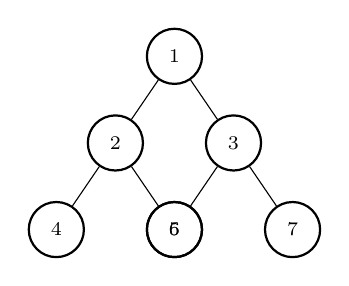
\begin{tikzpicture}[
  nodo/.style={draw=black, thick, circle, minimum size=7mm, font=\scriptsize},
  level distance=11mm, sibling distance=15mm
]
\node[nodo] {1}
  child { node[nodo] {2}
    child { node[nodo] {4} }
    child { node[nodo] {5} }
  }
  child { node[nodo] {3}
    child { node[nodo] {6} }
    child { node[nodo] {7} }
  };
\end{tikzpicture}

\small\textit{BFS: orden de expansión 1,2,3,4,5,6,7 (nivel por nivel).}
\end{minipage}
\hfill
\begin{minipage}{0.48\textwidth}
\centering
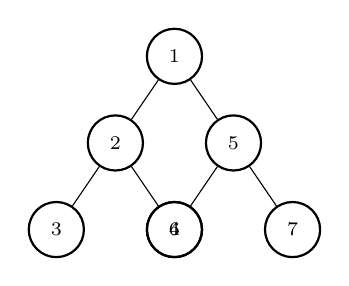
\begin{tikzpicture}[
  nodo/.style={draw=black, thick, circle, minimum size=7mm, font=\scriptsize},
  level distance=11mm, sibling distance=15mm
]
\node[nodo] {1}
  child { node[nodo] {2}
    child { node[nodo] {3} }
    child { node[nodo] {4} }
  }
  child { node[nodo] {5}
    child { node[nodo] {6} }
    child { node[nodo] {7} }
  };
\end{tikzpicture}

\small\textit{DFS: orden de expansión 1,2,3,4,5,6,7 (baja hasta el fondo antes de retroceder).}
\end{minipage}
\caption{Mismo árbol de búsqueda, dos órdenes de expansión distintos según la estructura de datos de la frontera
(cola FIFO en BFS, pila LIFO en DFS).}
\end{figure}

\subsection{Depth-Limited Search y Iterative Deepening (IDDFS)}

IDDFS ejecuta DFS con límite de profundidad creciente $l = 0, 1, 2, \ldots$

\begin{itemize}
    \item Combina las ventajas de BFS (completo, óptimo si costos iguales) con las de DFS (espacio lineal).
    \item Tiempo: $\bigO{b^d}$ \quad Espacio: $\bigO{bd}$
\end{itemize}

\subsection{Uniform-Cost Search (UCS)}

\begin{itemize}
    \item Expande el nodo con menor \textbf{costo de camino} $g(n)$ (cola de prioridad).
    \item Equivale a BFS cuando todos los costos son iguales.
    \item \textbf{Completo}: sí (si costos $> \epsilon > 0$).
    \item \textbf{Óptimo}: sí.
    \item Tiempo y espacio: $\bigO{b^{1+\lfloor C^*/\epsilon \rfloor}}$, donde $C^*$ es el costo óptimo.
\end{itemize}

\begin{example}[UCS sobre un grafo con costos]
    Usando el grafo de Rumania de la clase anterior, para ir de $Arad$ a $Bucarest$, UCS explora en este orden (por
    costo acumulado $g(n)$ creciente): $Arad(0)$, $Zerind(75)$, $Sibiu(140)$, $Oradea(146)$, $Rimnicu(220)$,
    $Fagaras(239)$, $Bucarest$ vía $Rimnicu \to Pitesti \to Bucarest$ con costo $418$, que resulta más barato que ir
    vía $Fagaras$ (costo $450$), aunque $Fagaras$ se alcance primero.
\end{example}

\subsection{Comparativa Búsqueda Desinformada}

\begin{center}
\begin{tabular}{lcccc}
\toprule
\textbf{Algoritmo} & \textbf{Completo} & \textbf{Óptimo} & \textbf{Tiempo} & \textbf{Espacio} \\
\midrule
BFS      & Sí & Sí* & $b^d$     & $b^d$ \\
DFS      & No & No  & $b^m$     & $bm$ \\
IDDFS    & Sí & Sí* & $b^d$     & $bd$ \\
UCS      & Sí & Sí  & $b^{C^*/\epsilon}$ & $b^{C^*/\epsilon}$ \\
\bottomrule
\multicolumn{5}{l}{\small *Óptimo si costos de paso son iguales}
\end{tabular}
\end{center}
